When a string is plucked, it will create travelling waves on the string that reflect at both ends, creating standing waves. The frequency of the wave with the longest wavelength is the fundamental frequency, also called the first harmonic. This is the lowest frequency, and there will usually be other higher harmonics that when combined create the characteristic timbre of the electric guitar.
The fundamental frequency $f_0$ of a string can be determined by Mersenne's law:
\begin{equation}\label{eqn1}
    f_0 = \frac{1}{2l_s}\sqrt{\frac{T}{\mu}}
\end{equation}
where $l_s$ is the vibrating length of the string, $T$ is the tension, and $\mu$ is the linear density of the string (mass of string per unit length). \cite{mersenne} \par
When the string is fretted and plucked, its vibrating length changes, changing the frequency. Figure \ref{fig2} shows a model of the string pressed down on fret $n$. The distance from the bridge to the fret then is $l_n$.

\begin{figure}[!htbp]
    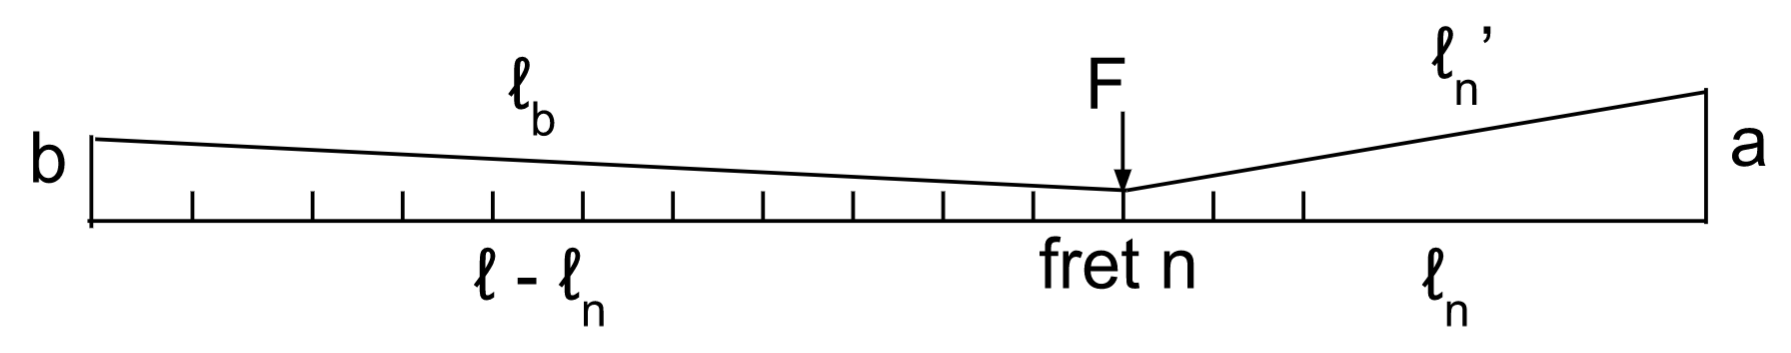
\includegraphics[width=\textwidth]{./ee/fig3.png}
    \caption{A simplified model of the fretted string}\label{fig2}
\end{figure}
In Western music, the ubiquitous musical system is the twelve-tone equal temperament (12-TET) system, where an octave is divided into 12 equally spaced notes on a logarithmic scale \cite{yuval}. The ratio is thus equal to $\sqrt[12]{2}$; therefore, to position the frets correlating to the notes, the scale length\footnote{Distance between the nut and the bridge} $l$ needs to be divided into powers of $\sqrt[12]{2}$. To calculate the position of each fret, luthiers traditionally use this formula. \cite{eqn6}
\begin{equation}\label{eqn2}
    l_n=\frac{l}{2^\frac{n}{12}}
\end{equation}